\documentclass{beamer}
\usepackage{graphicx}
\usepackage{booktabs}
\usepackage{graphicx}
\usepackage{subcaption}
\usepackage{caption}
\usepackage{tikz}
\usetikzlibrary{positioning}
\usepackage{graphicx}
\usepackage{subcaption}
\usepackage{caption}
\usepackage{adjustbox}
\usepackage{graphicx}
% \usetheme{Madrid}
% \usecolortheme{seahorse}
\usetheme{CambridgeUS}
\usecolortheme{crane}

\graphicspath{{./a/}}

\title{Unsupervised Domain Adaptation}
\author{}
\institute{Indian Institute of Science, Bangalore}
\date{\today}

\begin{document}

% Title Slide
\frame{\titlepage}

\begin{frame}
    \frametitle{Project Motivation}
    Our goal is to explore the field of \textbf{Unsupervised Domain Adaptation (UDA)} and Implement some of the state-of-the-art methods.\\
    Flow of the presentation:
    \begin{itemize}
        \item Introduction to UDA
        \item Domain-Adversarial Training of Neural Networks (DANN)
        \item Survey of Other Methods of UDA
        \begin{itemize}
            \item Divergence Based Methods
            \item Reconstruction Based Methods
            \item Ensemble Methods
        \end{itemize}
    \end{itemize}    

\end{frame}

\begin{frame}
    \frametitle{What is UDA?}
    \textbf{Domain Adaptation (DA)} is a subfield of machine learning that focuses on transferring knowledge from a source domain to a target domain with different data distributions.\\
    \textbf{Key Idea:} The goal is to learn a model that performs well on the target domain, even when only labeled data from the source domain is available.\\
    \textbf{Challenges:} The main challenge in UDA is the domain shift, which occurs when the source and target domains have different distributions. This can lead to poor performance of standard learning techniques.\\
    \begin{figure}
        \centering
        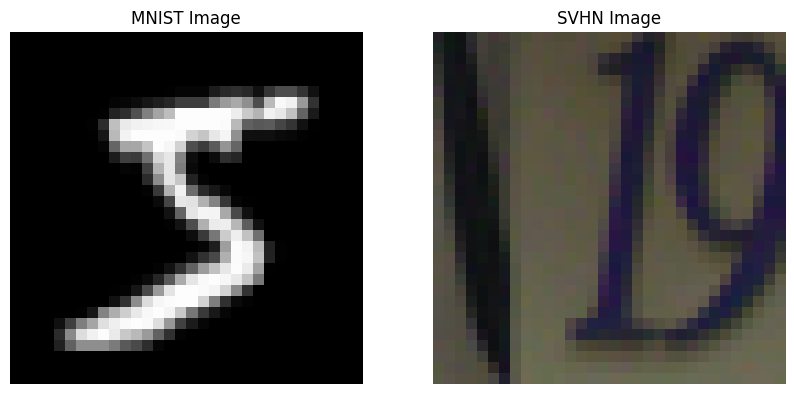
\includegraphics[width=0.5\linewidth]{Example of Domain Shift.png}
        \caption{Example of domain shift between source and target domains}
    \end{figure}
\end{frame}

\begin{frame}
    \frametitle{What is UDA?}
    In \textbf{Unsupervised Domain Adaptation (UDA)}, only the source domain data is labeled, while the target domain data is unlabeled.\\

    \textbf{Applications:} 
    \begin{itemize}
        \item When shifting a model trained on \textbf{synthetic data} to \textbf{real-world data}, the model may not perform well due to the differences in data distributions.
        \item For systems like \textbf{Security Cameras} and \textbf{Autonomous Driving}, the inputs to each camera belong to different domains. So we wish to adapt the model to the new domain.
    \end{itemize}

    

\end{frame}
% % Slide 1 - Motivation
% \begin{frame}{Project Motivation}

% \begin{itemize}
%     \item \textbf{Domain adaptation} aims to transfer knowledge from a source domain to a target domain with different data distributions.
%     \item In the \textbf{unsupervised} setting, only source domain data is labeled; target domain data is unlabeled.
%     \item Standard learning techniques fail due to the \textbf{domain shift}.
%     \item To address this, we train models to learn \textbf{domain-invariant features} that perform well across domains.
% \end{itemize}
% \end{frame}

% % Slide 2 - Setup
% \begin{frame}{Domain Adaptation Setup}
% \begin{itemize}
%     \item Input space: $\mathcal{X}$, Label space: $\mathcal{Y} = \{0, 1, \ldots, L-1\}$
%     \item \textbf{Source distribution:} $\mathcal{D}_S$ over $\mathcal{X} \times \mathcal{Y}$
%     \item \textbf{Target distribution:} $\mathcal{D}_T$ over $\mathcal{X} \times \mathcal{Y}$
%     \item Training data:
%     \begin{itemize}
%         \item Labeled source set: $S = \{(x_i, y_i)\}_{i=1}^{n}$
%         \item Unlabeled target set: $T = \{x_j\}_{j=1}^{n'}$
%     \end{itemize}
% \end{itemize}
% \end{frame}

% % Slide 3 - H-Divergence
% \begin{frame}{$\mathcal{H}$-Divergence}
% \[
% d_{\mathcal{H}}(\mathcal{D}_S^X, \mathcal{D}_T^X) = 2 \sup_{\eta \in \mathcal{H}} \left| \Pr_{x \sim \mathcal{D}_S^X}[\eta(x)=1] - \Pr_{x \sim \mathcal{D}_T^X}[\eta(x)=1] \right|
% \]

% \begin{itemize}
%     \item Measures the ability of a hypothesis $\eta \in \mathcal{H}$ to distinguish between source and target distributions.
%     \item High $d_{\mathcal{H}}$ implies easy domain discrimination — bad for transfer.
%     \item For symmetric hypothesis classes, it can be estimated via:
%     \[
%     \hat{d}_A = 2 (1 - 2\epsilon)
%     \]
%     \item Here, $\epsilon$ is the generalization error of a domain classifier.
% \end{itemize}
% \end{frame}

% Slide 4 - DANN Architecture
\begin{frame}{DANN Architecture}
\begin{figure}
    \centering
    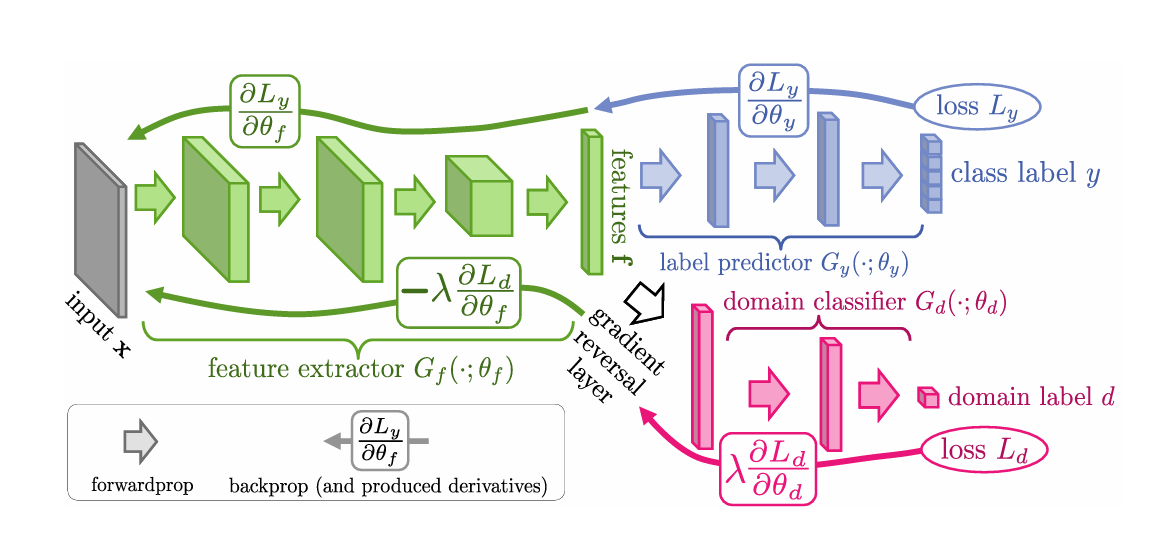
\includegraphics[width=0.9\linewidth]{DANN_img.png}
    \caption{Domain-Adversarial Neural Network (DANN) Architecture}
\end{figure}
\end{frame}

\begin{frame}
    \frametitle{DANN}
    
    

\end{frame}

% Slide 5 - Key Idea
\begin{frame}{DANN: Key Idea}
\begin{itemize}
    \item Simultaneous optimization of:
    \begin{enumerate}
        \item \textbf{Label predictor} — classifies source data correctly
        \item \textbf{Domain classifier} — fails to distinguish source from target
    \end{enumerate}
    \item The \textbf{feature extractor} is trained to:
    \begin{itemize}
        \item Minimize label prediction loss (task objective)
        \item Maximize domain classification loss (encourages invariance)
    \end{itemize}
\end{itemize}
\end{frame}

% Slide 6 - Architecture Overview
\begin{frame}{DANN Architecture Overview}
\begin{itemize}
    \item \textbf{Feature extractor} $G_f$: shared across tasks
    \item \textbf{Label predictor} $G_y$: trained on labeled source data
    \item \textbf{Domain classifier} $G_d$: trained to classify domain
    \item \textbf{Gradient Reversal Layer (GRL)}: connects $G_f$ and $G_d$
\end{itemize}
\end{frame}

% Slide 7 - GRL
\begin{frame}{Gradient Reversal Layer (GRL)}
\begin{itemize}
    \item \textbf{Forward pass:} identity function: $R(x) = x$
    \item \textbf{Backward pass:} gradient scaled by $-\lambda$: 
    \[
    \frac{dR}{dx} = -\lambda I
    \]
    \item GRL enables adversarial training by reversing gradients from the domain classifier.
    \item This pushes $G_f$ to generate domain-invariant features.
\end{itemize}
\end{frame}

% Slide 8 - Objective Function
\begin{frame}{Objective Function}
\[
\min_{\theta_f, \theta_y} \max_{\theta_d} \mathcal{E}(\theta_f, \theta_y, \theta_d)
\]
\vspace{-1em}
\[
\mathcal{E} = \frac{1}{n} \sum_{i=1}^{n} L_y(G_y(G_f(x_i)); y_i) 
- \lambda \sum_{j=1}^{n+n'} L_d(G_d(G_f(x_j)); d_j)
\]
\begin{itemize}
    \item \textbf{Label loss:} minimized w.r.t. $\theta_f$, $\theta_y$
    \item \textbf{Domain loss:} maximized w.r.t. $\theta_f$, minimized w.r.t. $\theta_d$
    \item $\lambda$ balances the two objectives
\end{itemize}
\end{frame}

\begin{frame}{Experiments}
The experiments section is divided into 3 parts: 
\begin{itemize}
    \item Experiments on shallow DNN
    \item Experiments on image classification
    \item Experiments on image reconstruction
\end{itemize}
    
\end{frame}


\begin{frame}{Experiments on Shallow DNN}
\vspace{-0.2cm}

\textbf{Intertwining moons}: Dataset used for evaluating domain adaptation.\\[0.2cm]
The structure of source and target distributions is shown below:

\vspace{0.5cm}

\begin{center}
    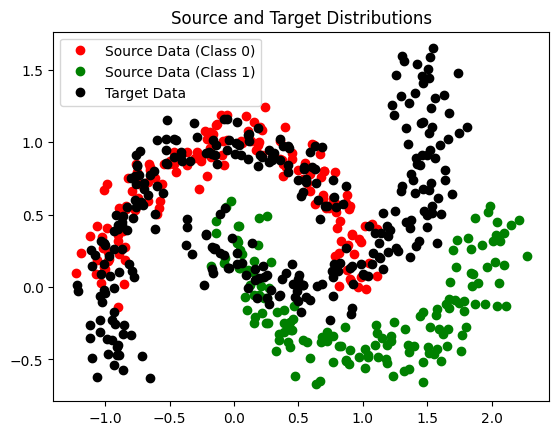
\includegraphics[width=0.7\linewidth]{moon.png}
    \captionof{figure}{\small\textbf{Source and Target Distributions}. \textcolor{red}{Red} and \textcolor{green!70!black}{green} points represent source data (Class 0 and 1, respectively), while \textcolor{black}{black} points are from the target domain.}
\end{center}

\end{frame}

% \begin{frame}{Results on the inter-twinning moons problem}
% \centering

% % --- First Row: Standard NN ---
% \begin{figure}
% \centering
% \begin{subfigure}[t]{0.30\linewidth}
%     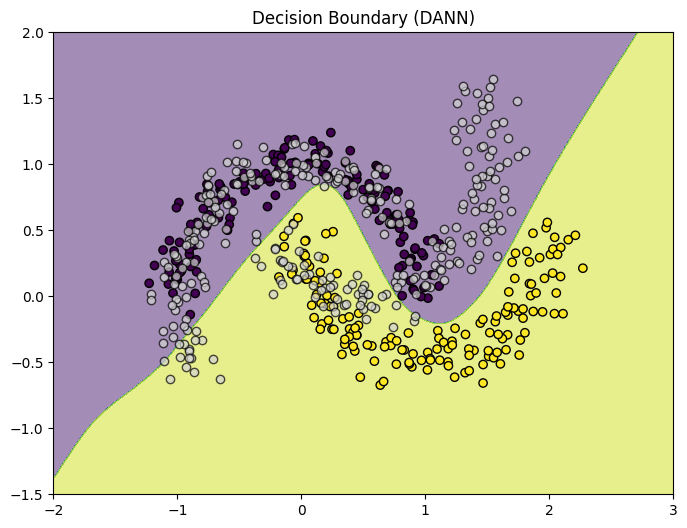
\includegraphics[width=\linewidth]{label_decision_vanilla.png}
%     \caption*{\small Label Classification}
% \end{subfigure}
% \hfill
% \begin{subfigure}[t]{0.30\linewidth}
%     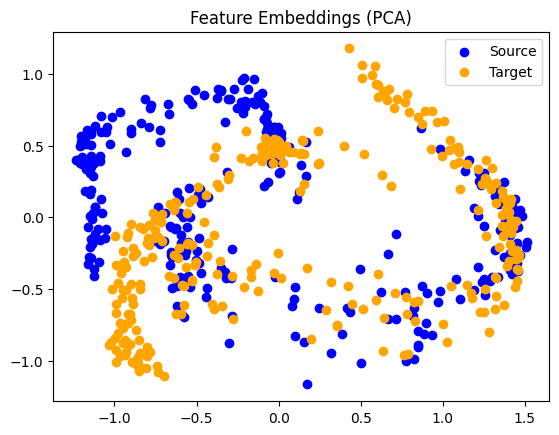
\includegraphics[width=\linewidth]{feature_vanilla.png}
%     \caption*{\small Representation PCA}
% \end{subfigure}
% \hfill
% \begin{subfigure}[t]{0.30\linewidth}
%     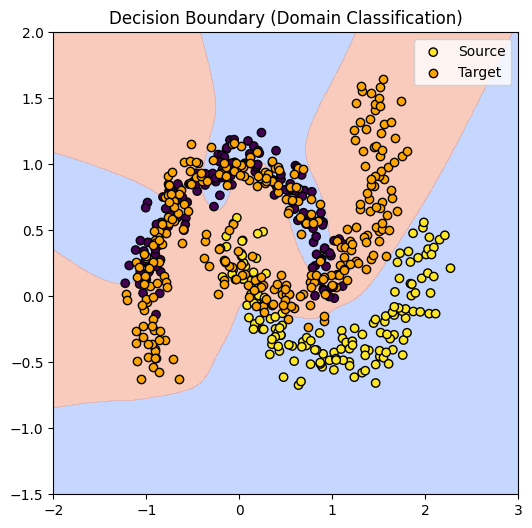
\includegraphics[width=\linewidth]{domain_deciison_vanilla.png}
%     \caption*{\small Domain Classification}
% \end{subfigure}
% \caption{(a) Standard NN}. 
% \end{figure}

% %\vspace{0.8cm}

% % --- Second Row: DANN ---
% \begin{figure}
% \centering
% \begin{subfigure}[t]{0.30\linewidth}
%     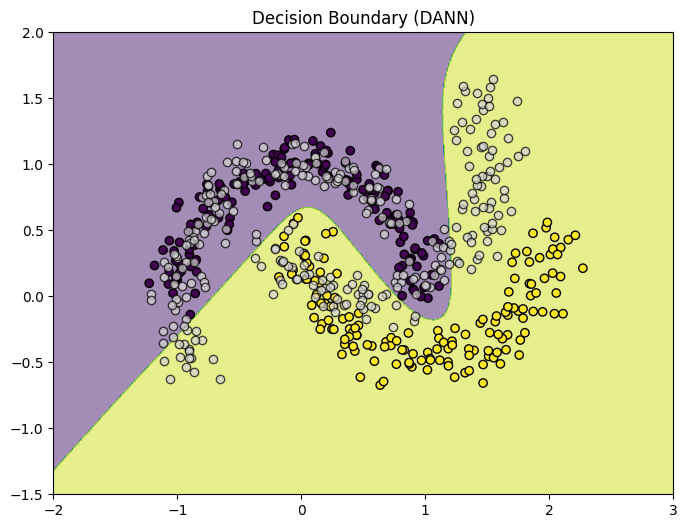
\includegraphics[width=\linewidth]{label_decision_dann.png}
%     \caption*{\small Label Classification}
% \end{subfigure}
% \hfill
% \begin{subfigure}[t]{0.30\linewidth}
%     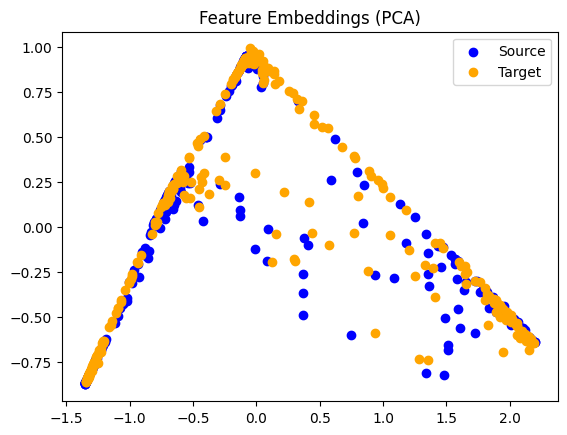
\includegraphics[width=\linewidth]{feature_dann.png}
%     \caption*{\small Representation PCA}
% \end{subfigure}
% \hfill
% \begin{subfigure}[t]{0.30\linewidth}
%     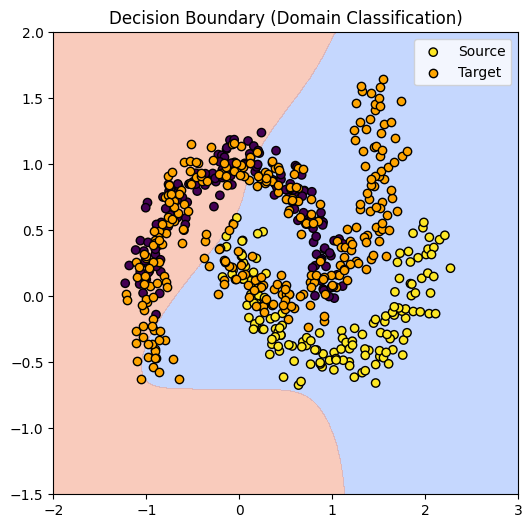
\includegraphics[width=\linewidth]{domain_decision_dann.png}
%     \caption*{\small Domain Classification}
% \end{subfigure}
% \caption{(b) DANN (Algorithm 1)}
% \end{figure}

% \end{frame}


\begin{frame}{Results on the inter-twinning moons problem}
\footnotesize
\centering

% --------- First Row: Standard NN -----------
\begin{minipage}{0.8\linewidth}
\centering
\begin{adjustbox}{max width=\textwidth}
\begin{tabular}{ccc}
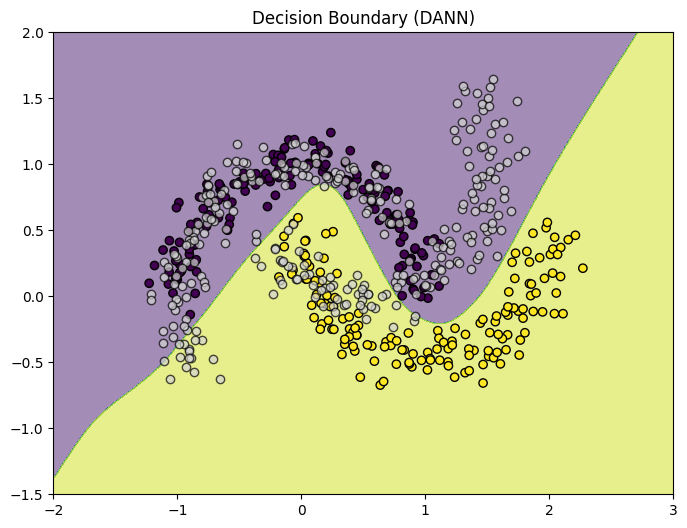
\includegraphics[width=0.3\textwidth]{label_decision_vanilla.png} &
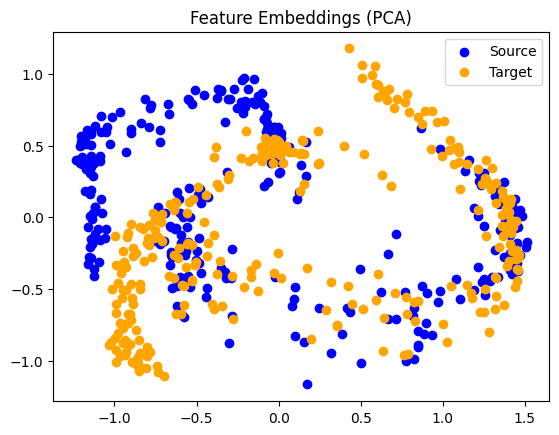
\includegraphics[width=0.3\textwidth]{feature_vanilla.png} &
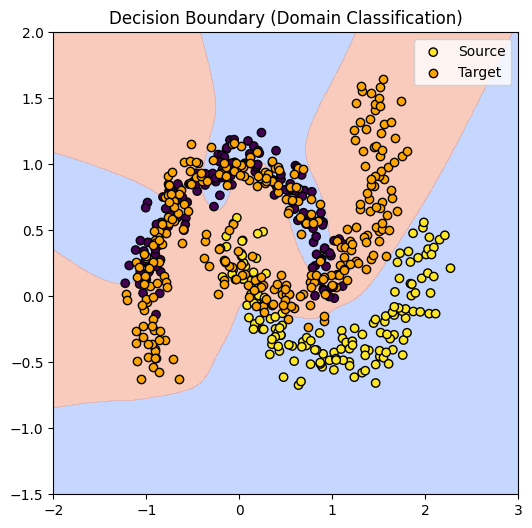
\includegraphics[width=0.3\textwidth]{domain_deciison_vanilla.png} \\
\small Label Classification & \small Representation PCA & \small Domain Classification
\end{tabular}
\end{adjustbox}
\end{minipage}

\vspace{0.0 cm}
\centering
\small\textbf{(a)} Standard NN.

\vspace{0.8cm}

% --------- Second Row: DANN -----------
\begin{minipage}{0.8\linewidth}
\centering
\begin{adjustbox}{max width=\textwidth}
\begin{tabular}{ccc}
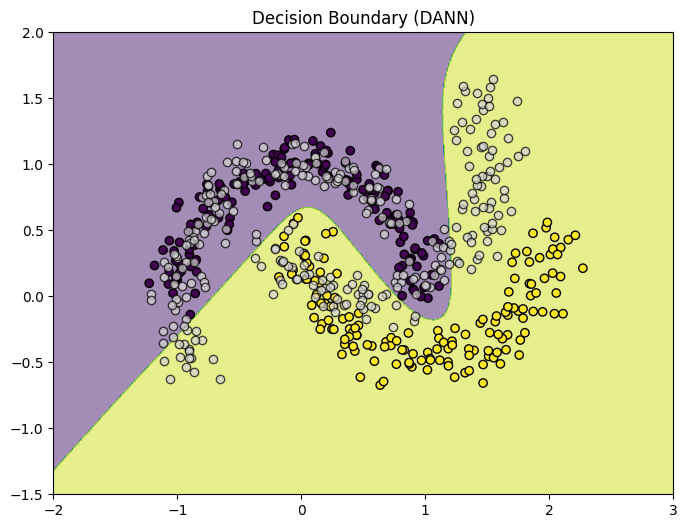
\includegraphics[width=0.3\textwidth]{label_decision_dann.png} &
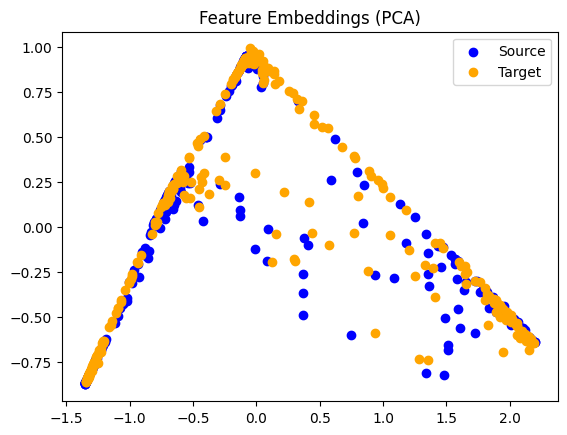
\includegraphics[width=0.3\textwidth]{feature_dann.png} &
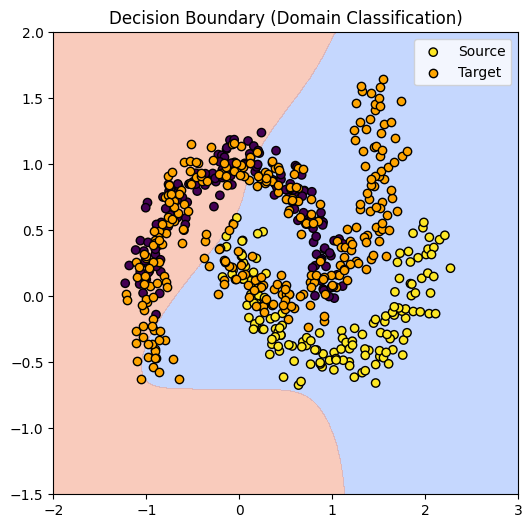
\includegraphics[width=0.3\textwidth]{domain_decision_dann.png} \\
\small Label Classification & \small Representation PCA & \small Domain Classification
\end{tabular}
\end{adjustbox}
\end{minipage}

\vspace{0.3cm}
\centering
\small\textbf{(b)} DANN

\end{frame}

% \begin{frame}{\centering \large MNIST $\rightarrow$ MNIST-M: Top Feature Extractor Layer}
% \centering

% \begin{adjustbox}{max width=\textwidth}
% \begin{tabular}{cc}
% % Left Image
% \begin{subfigure}[t]{0.45\textwidth}
%     \centering
%     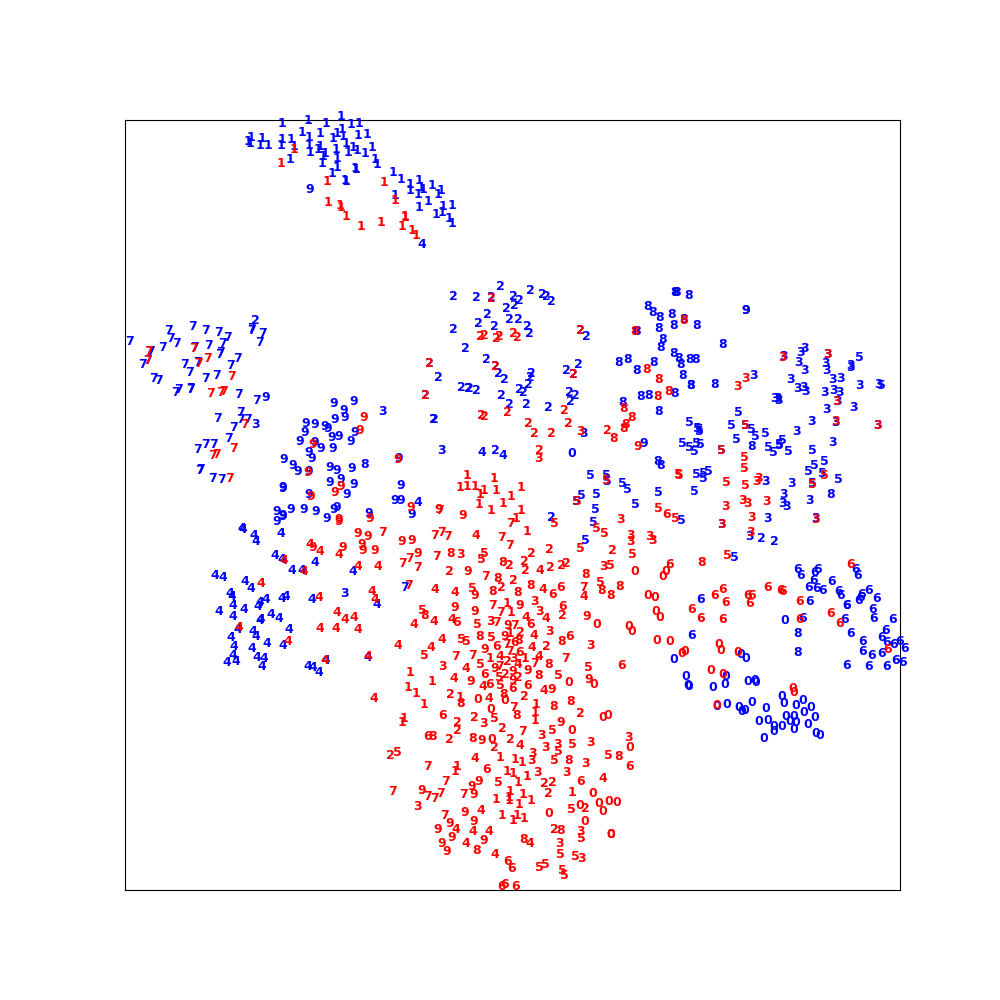
\includegraphics[width=\linewidth]{Source-only.png}
%     \caption{Non-adapted}
% \end{subfigure}
% &
% % Right Image
% \begin{subfigure}[t]{0.45\textwidth}
%     \centering
%     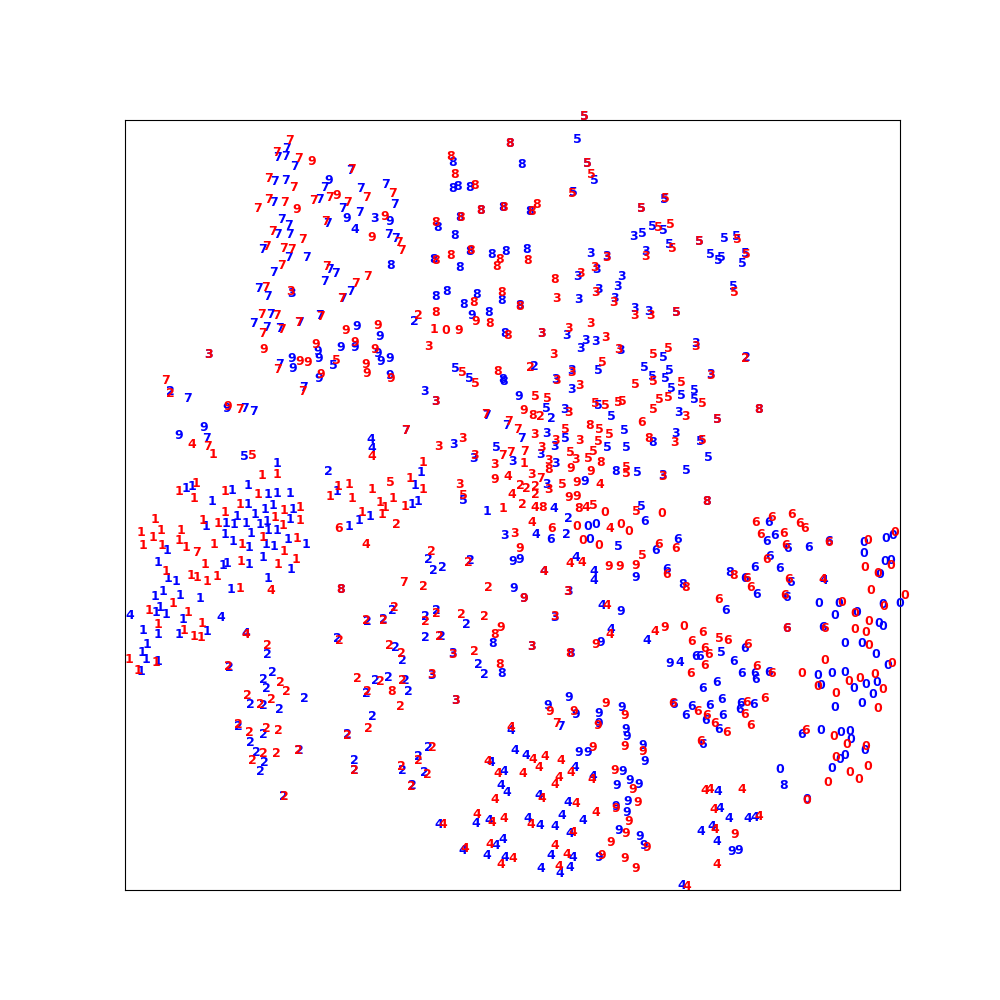
\includegraphics[width=\linewidth]{DANN.png}
%     \caption{Adapted}
% \end{subfigure}
% \end{tabular}
% \end{adjustbox}

% \vspace{0.3cm}
% \small
% \textbf{Figure:} t-SNE visualizations of extracted features. \textcolor{blue}{Blue} points: source domain (MNIST); \textcolor{red}{Red} points: target domain (MNIST-M). Adaptation aligns distributions better.

% \end{frame}

\begin{frame}
    \frametitle{Ensemble Methods}

    \textbf{Motivation:} Motivation of an Ensemble method is to use multiple diffrent models and then combine them to get a better performance. 
    We belive that mistakes from different averages out giving an overall better performance. \\

    \textbf{Methods used:} \\
    For Combining the results from the different models we have used the following methods: 
    \begin{itemize}
        \item \textbf{Majority Voting [Classification]:} The class with the most votes is selected as the final prediction.
        \item \textbf{Average [Regression]:} The average of the predictions is taken as the final prediction.
    \end{itemize}
    To obtain independent models we can do the following:
    \begin{itemize}
        \item Use different architectures for each model.
        \item Use different initializations for each model.
        \item Save instances of models on regular intervals while training.
    \end{itemize}

    

\end{frame}

\begin{frame}
    \frametitle{Asymmetric Tri-training}

    Ensemble model approach to UDA. Utilizing a feature extractor \(F\) and three classifiers \(F_1,F_2,F_t\).\\
    \textbf{Key Idea:} Use two classifiers to pseudo-label the target domain and train a third classifier on the pseudo-labeled data.\\


    \begin{figure}[h]
        \centering
        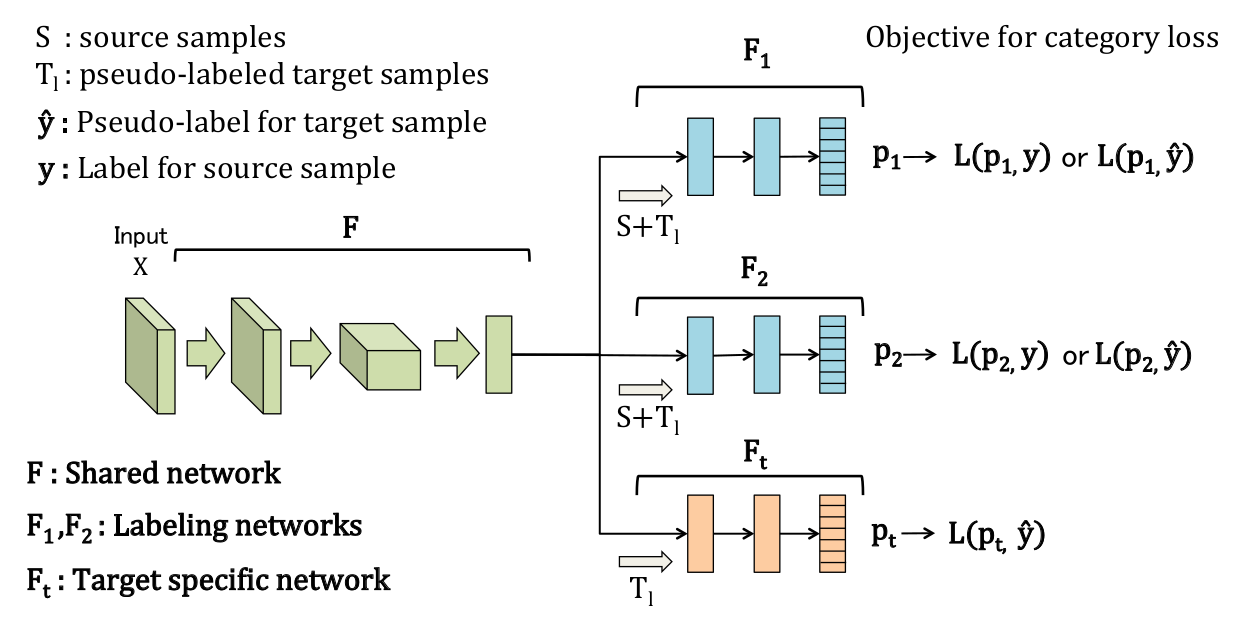
\includegraphics[width=0.9\linewidth]{ATT_achi.png}
        \caption{Asymmetric Tri-training Network Architecture}
    \end{figure}
\end{frame}

\begin{frame}
    \frametitle{MNIST - SVHN Domain Adaptation}
    \textbf{Dataset:} MNIST and SVHN are two datasets used for image classification. MNIST contains handwritten digits, while SVHN contains street view house numbers.\\

    \begin{figure}[h]
        \centering
        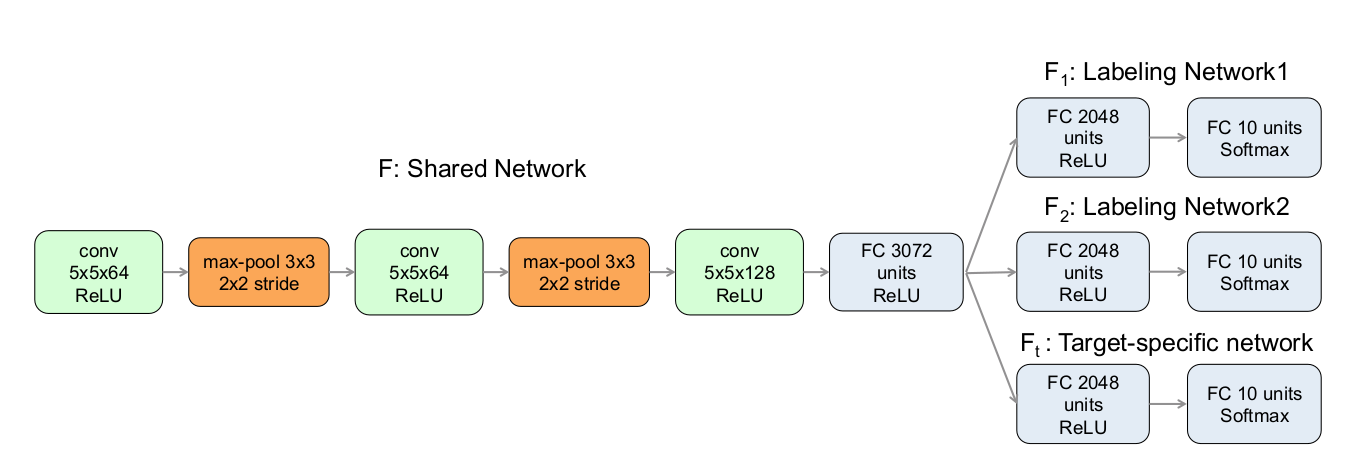
\includegraphics[width=0.9\linewidth]{att-msvhn-a.png}
        \caption{The architecture used for training SVHN}
    \end{figure}

\end{frame}

\begin{frame}{Algorithm Overview}
    \begin{columns}
      % Left column for text
      \begin{column}{0.5\textwidth}
        \small % adjust text size if needed
        \textbf{Key Points:}
        \begin{itemize}
          \item \textbf{Loss Function for F1 and F2:}
          \tiny \[
            \begin{aligned}
            \mathcal{L}_{\Theta_F,\Theta_{F1},\Theta_{F2}} &= \frac{1}{n} \sum_{i=1}^{n} [L_y(F_1(F(x_i)); y_i)\\ &+ L_y(F_2(F(x_i)); y_i)] \\
            &+ \lambda |W_1^T W_2|
            \end{aligned}
          \]
        \end{itemize}
      \end{column}
    
      % Right column for the image
      \begin{column}{0.5\textwidth}
        \centering
        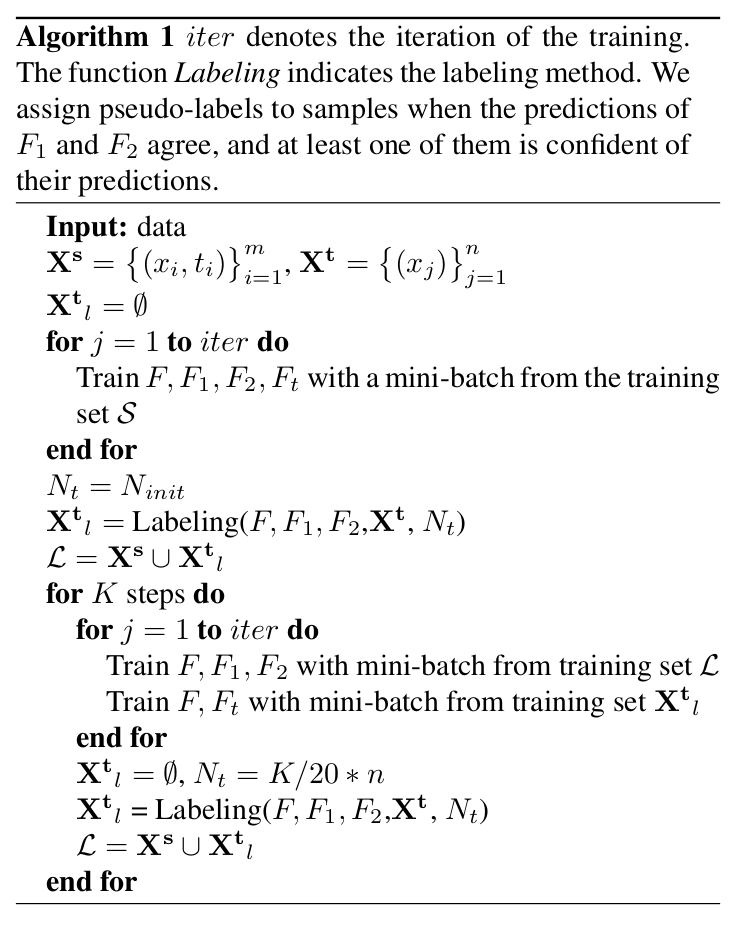
\includegraphics[width=\textwidth]{algo_att.png}
      \end{column}
    \end{columns}
\end{frame}

\begin{frame}
    \frametitle{Results of ATT on MNIST and SVHN Domain Adaptation}

    \begin{table}[h]
        \centering
        \caption{Results of ATT on MNIST and SVHN Domain Adaptation.}
        \label{tab:att_results}
        \begin{tabular}{lccc}
            \toprule
            \textbf{Method} & \textbf{MNIST\(\to\)SVHN} & \textbf{SVHN \(\to\) MNIST} \\
            \midrule
            Our w/o Batch Normalization & 36.9\% & 76.8\% \\
            Ours w/o Multi-view Loss & 15.2\% & 76.5\% \\
            Ours  & 15.2\% & 71.4\% \\
            \midrule
            Papers w/o Batch Normalization & 39.8\% & 79.8\% \\
            Papers w/o Multi-view Loss & 49.7\% & 86.0\% \\
            Papers  & 52.8\% & 85.8\% \\
            \bottomrule
        \end{tabular}
      \end{table}
\end{frame}


\begin{frame}
    \frametitle{Maximum Mean Discrepancy}
    \textbf{Concept:} MMD is a statistical test to measure the distance between two distributions. It is used to determine if two samples are drawn from the same distribution.\\
    \textbf{Key Idea:} MMD is defined as the squared distance between the mean embeddings of two distributions in a reproducing kernel Hilbert space (RKHS).\\
    \textbf{Mathematical Definition:}
    \[
        \text{MMD}^2(\mathcal{D}_S, \mathcal{D}_T) = \left\| \frac{1}{n} \sum_{i=1}^{n} \phi(x_i) - \frac{1}{m} \sum_{j=1}^{m} \phi(y_j) \right\|_{\mathcal{H}}^2
    \]
    \[
        \text{MMD}^2_k(P,Q) := \mathbb{E}_{x,x'}[k(x,x')] + \mathbb{E}_{y,y'}[k(y,y')] - 2\mathbb{E}_{x,y}[k(x,y)]
    \]   
\end{frame}

\begin{frame}
    \frametitle{Estimation of MMD}
    MMD can be estimated using the empirical distributions of the samples. The empirical MMD is given by:
    \[
         X = \{x_1, x_2, \ldots, x_n\} \text{ and } Y = \{y_1, y_2, \ldots, y_m\}
    \]
    \small \[
        \hat{\text{MMD}}^2(X,Y) = \frac{1}{n(n-1)} \sum_{i \neq j} k(x_i, x_j) + \frac{1}{m(m-1)} \sum_{i \neq j} k(y_i, y_j) - \frac{2}{nm} \sum_{i,j} k(x_i, y_j)
    \]
    From this we can define a test statistic:
    \[
        T = \frac{\hat{\text{MMD}}^2(X,Y)}{\sqrt{\hat{V_m}(X,Y)}}
    \]
    Where \(V_m\) is unbiased estimator of the variance of the MMD.\\
    \textbf{Key Idea:} If \(T\) is large, then the two distributions are likely different.\\

\end{frame}

\begin{frame}
    \frametitle{Experiments on MMD}
    We have used synthetic data to test MMD. The experiment uses two different distributions:
    \begin{figure}[h]
        \centering
        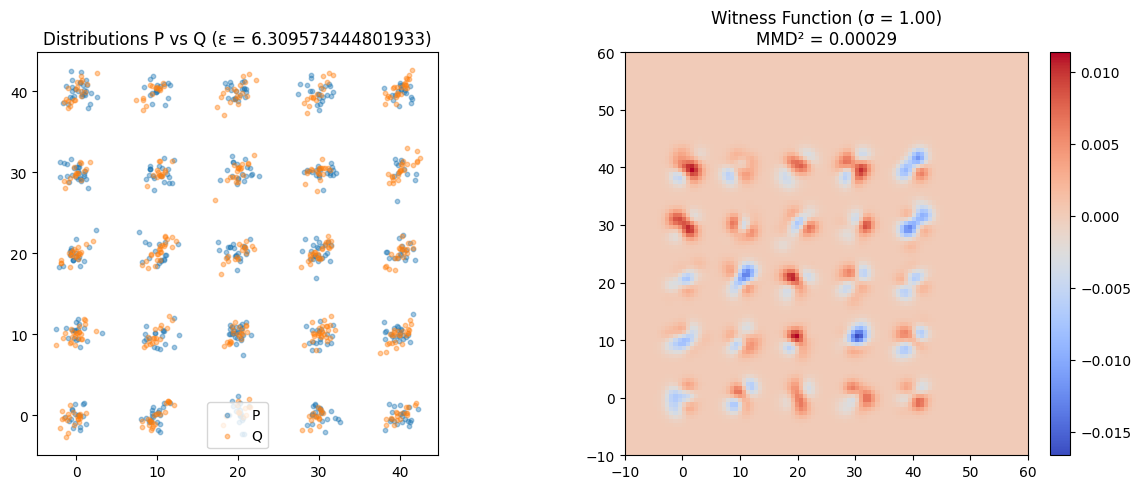
\includegraphics[width=0.9\linewidth]{mmdDataset.png}
        \caption{Synthetic datasets used for MMD experiments.}
    \end{figure}
\end{frame}

\begin{frame}
    \frametitle{Results of MMD}
    \begin{figure}[h]
        \centering
        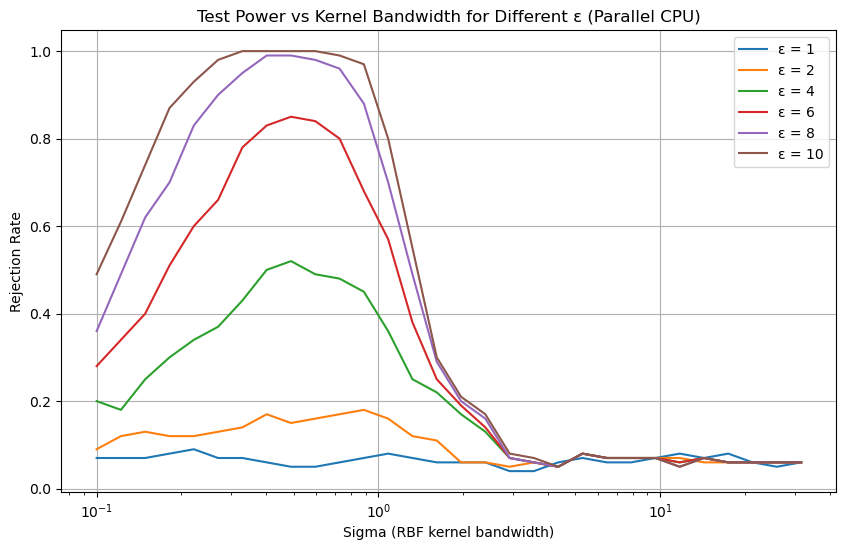
\includegraphics[width=0.8\linewidth]{Test_powe_vs_eps.png}
        \caption{Test power vs $\epsilon$ (epsilon). As the difference between distributions increases, MMD becomes more effective at distinguishing them.}
    \end{figure}
\end{frame}

\begin{frame}
    \frametitle{Results of MMD}

    \begin{figure}[h]
        \centering
        \begin{minipage}{0.48\textwidth}
            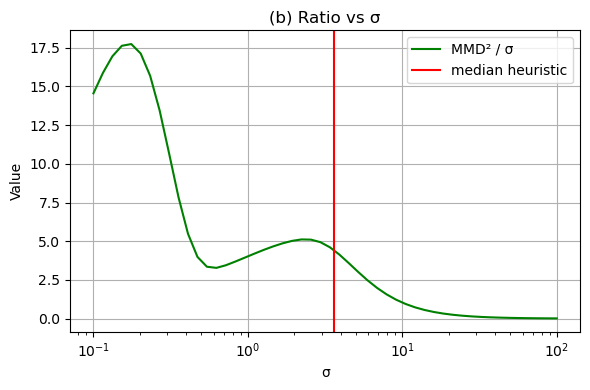
\includegraphics[width=\linewidth]{t_vs_sigma.png}
            \caption{Test statistic T vs kernel bandwidth $\sigma$}
        \end{minipage}
        \hfill
        \begin{minipage}{0.48\textwidth}
            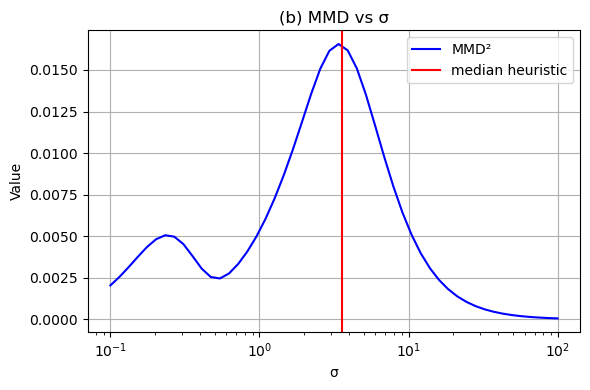
\includegraphics[width=\linewidth]{MMD vs sigma.png}
            \caption{MMD value vs kernel bandwidth $\sigma$}
        \end{minipage}
    \end{figure}
\end{frame}

\begin{frame}
    \frametitle{MMD use in UDA}
    \textbf{Key Idea:} MMD can be used as a loss function to minimize the distance between the source and target distributions.\\

    Methods:
    \begin{itemize}
        \item We can train Neural Networks using MMD as a loss function.
        \item We can combine multiple kernels using a weighted sum and learn their weights: 
        \[
        k(x,y) = \sum_{i=1}^m \beta_i k_i(x,y), \quad \beta_i \geq 0, \quad \sum_{i=1}^m \beta_i = 1
        \]
        \item We c
    \end{itemize}

    


\end{frame}


\end{document}
